\documentclass[a4paper,12pt,danish]{article}

\ProvidesPackage{setup}

\usepackage[utf8]{inputenc}

\usepackage[english]{babel}

\usepackage{fixltx2e}

\usepackage{graphicx}

\usepackage{lastpage}

\usepackage{fancyhdr}

\usepackage{multicol}

\usepackage[T1]{fontenc}

\usepackage[top=3cm, bottom=3cm, left=2.5cm, right=3.5cm]{geometry}

\usepackage{tocvsec2}

\usepackage{float}

\usepackage{tabularx}

\usepackage{parskip}

\usepackage{mathtools}

\usepackage{changepage}

\usepackage{gensymb}

\usepackage{mdwlist}

\usepackage{algorithm}

\usepackage{titlesec}

\usepackage{algpseudocode}

\usepackage{subfiles}

\usepackage{color}

\usepackage{hyperref}

\usepackage{booktabs}

%\usepackage{verbatim}

\algrenewcommand\algorithmicprocedure{\textbf{function}}

\usepackage[nottoc,numbib]{tocbibind}

\usepackage{setspace}

\usepackage{array}

\usepackage{lastpage}
\pagestyle{fancy}

\cfoot{\thepage\ of \pageref{LastPage}}
\renewcommand{\headrulewidth}{0pt}
\fancyhead{}

\titlespacing*{\section}{0pt}{0.5cm}{0cm}
\titlespacing*{\subsection}{0pt}{0.3cm}{0cm}
\titlespacing*{\subsubsection}{0pt}{0.1cm}{0cm}
\titlespacing*{\paragraph}{0pt}{0cm}{0cm}

\setcounter{secnumdepth}{4}

\titleformat{\paragraph}
{\normalfont\normalsize\bfseries}{\theparagraph}{1em}{}


\title{\textbf{Algorithms and Datastructures -- Tower Of Hanoi}}
\author{Stefan Ravn van Overeem – stvan13@student.sdu.dk \\
		Martin Staal Steenberg – mstee13@student.sdu.dk}

\begin{document}
\maketitle
\section{Implementation}
	We have implented a solution to the Tower of Hanoi Problem using recursion.
	The rods have been implemented as a class containing a list of discs on the rod, with functions to place new discs onto the top of the rod, and likewise remove discs from the top. Error checking is done to emit a error message if a large disc is placed on top of a smaller one.
	
	The Tower of Hanoi Game is likewise implemented as a class, containing three Rods.
	When the rods are constructed, a specified number of discs is placed upon the first rod, while the two others are left empty.
	A function, called solve is created, which calls the recursive function move\_discs, to solve the game.

\begin{algorithm}[H]
	\begin{algorithmic}[1]
		\Procedure{solve}{}
		\State this->MOVE\_DISCS(A, B, C, N)
		\EndProcedure
	\end{algorithmic}
	\caption{solve function}
\end{algorithm}


\begin{algorithm}[H]
	\begin{algorithmic}[1]
		\Procedure{MOVE\_DISCS}{Rod \&From, Rod \&To, Rod \&Last, int N}
		\If{N == 1} //Base case
		\State Pop top of \textit{From}, and push it onto \textit{To}.
		\State \Return
		\EndIf
		\State MOVE\_DISCS(From, Last, To, N - 1)
		\State MOVE\_DISCS(From, To, Last, 1)
		\State MOVE\_DISCS(Last, To, From, N - 1)
		\EndProcedure
	\end{algorithmic}
	\caption{move\_discs function}
\end{algorithm}
\newpage

The move\_discs function works by first moving the N - 1 top discs from the first rod to the last rod. This means that there now is only one disc left on the first rod, which then easily can be moved to the second and final rod. The discs moved to the last rod is then moved to the final rod, completing the puzzle.

The function calls itself recursively, and reduces the number of discs to move down to one, which is then easily moved to the wanted rod.

\section{Time Complexity}
To solve the tower N disc have to be moved. For each $N-1$ disc that have to be moved the prior discs have to be moved and then placed back on top. Which means we get a time complexity of $\mathcal{O}(2^N)$.

    \begin{figure}[H]     
    	\centering
    	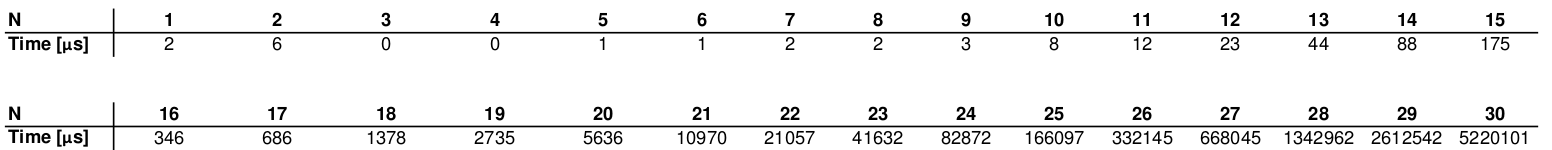
\includegraphics[width=\textwidth]{Times.png}
    	\caption{}
    	\label{timeTable}
    \end{figure}
    
    \begin{figure}[H]     
    	\centering
    	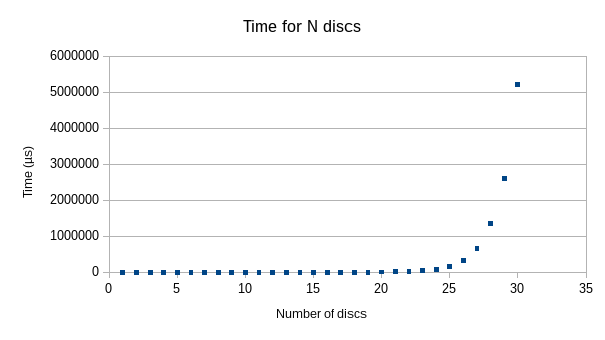
\includegraphics[width=\textwidth]{Time.png}
    	\caption{}
    	\label{time}
    \end{figure}
		

As can be seen on figure \ref{timeTable} and \ref{time}, the time doubles each time N is increased by one. This means that the expected time complexity of  $\mathcal{O}(2^N)$, is true for this implementation of the Tower of Hanoi.

The memory complexity of the program is equal to  $\mathcal{O}(N)$ because the only thing that have to be stored is the call stack and the rods, which is the size of $2 \cdot N$.
\section{Steps}
Steps taken by the algorithm with N = 5 can be seen on figure \ref{steps}


    \begin{figure}[H]     
    	\centering
    	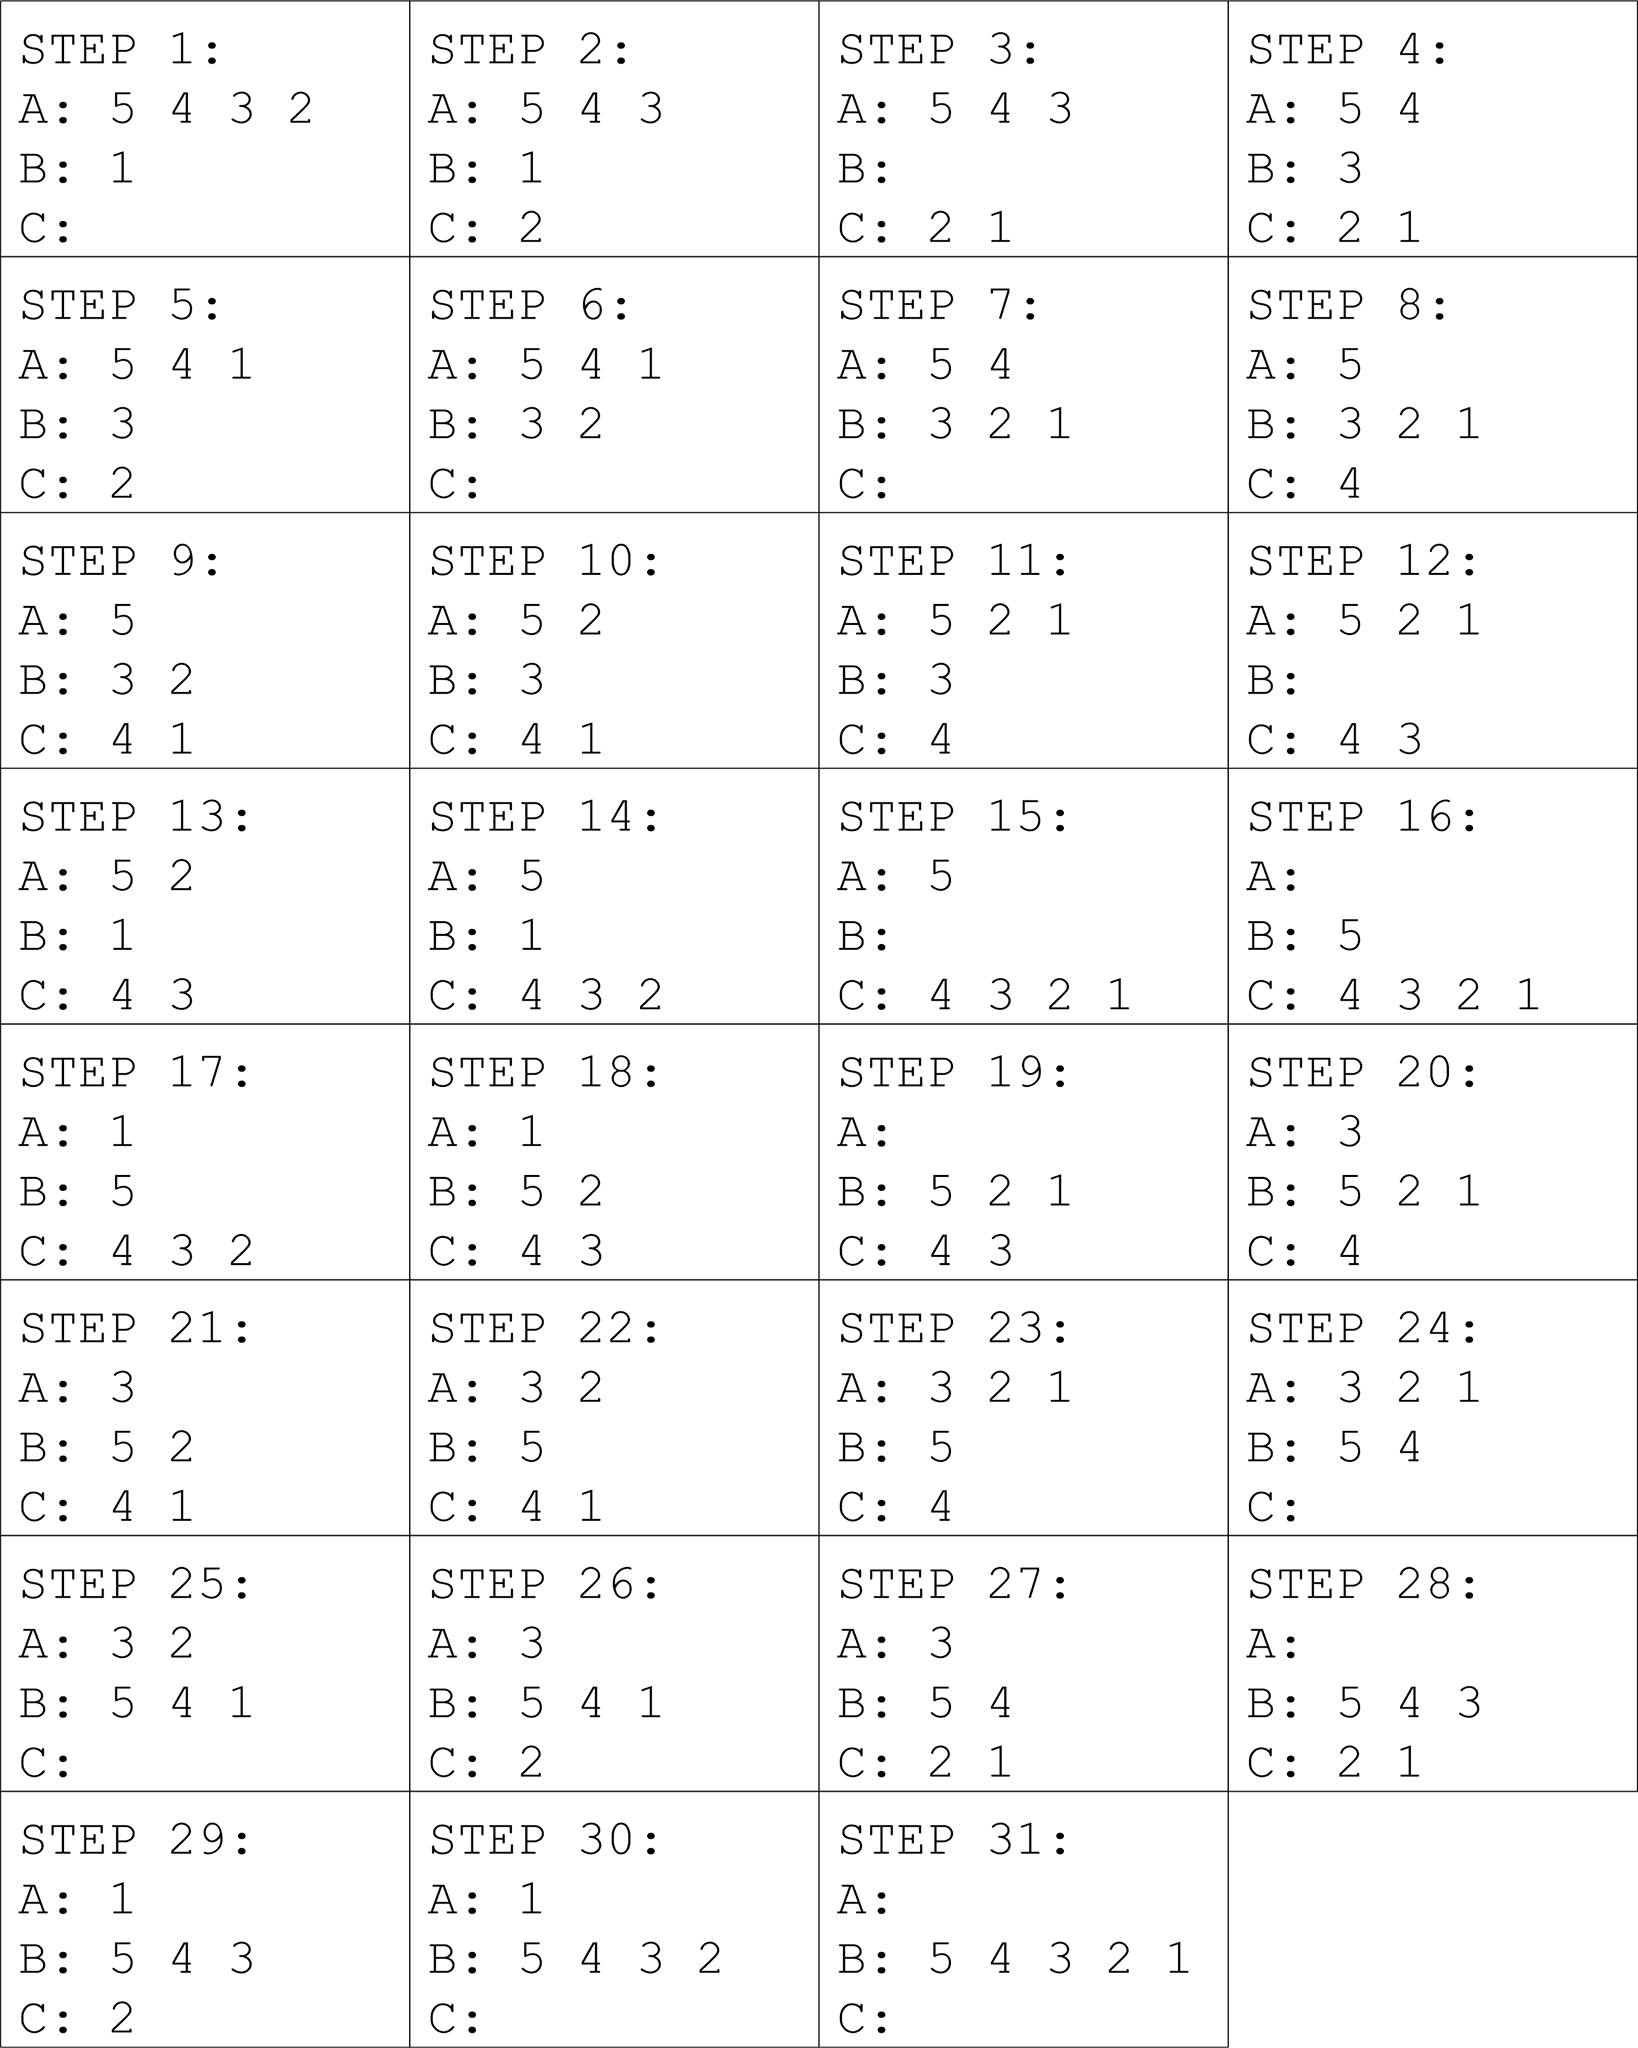
\includegraphics[width=\textwidth]{steps.jpg}
    	\caption{}
    	\label{steps}
    \end{figure}
    
\section{Code}
The code can be found on Github <https://github.com/StefanRvO/ADA/tree/master/Portfolio1>
The code can be compiled using cmake.
\end{document}